\chapter{Desenvolvimento}
\label{cap:desenvolvimento}

Este capítulo apresenta o desenvolvimento do estudo de caso com Microsserviços e \acrshort{ddd}. Ele descreve as etapas para construção do sistema a partir de requisitos funcionais e não-funcionais.

\section{Ciclo de Vida do Desenvolvimento de Software}
\citeonline{barbaraLiskov} descreve 6 etapas no ciclo de vida de um software: Análise de requisitos, \english{Design}, Implementação e Teste, Teste de aceitação, Produção e Manutenção. A Figura \ref{fig:ciclo-vida} ilustra essas etapas. 

\begin{figure}[H]
    \centering
    \caption{Ciclo de Vida do Desenvolvimento de Software}
    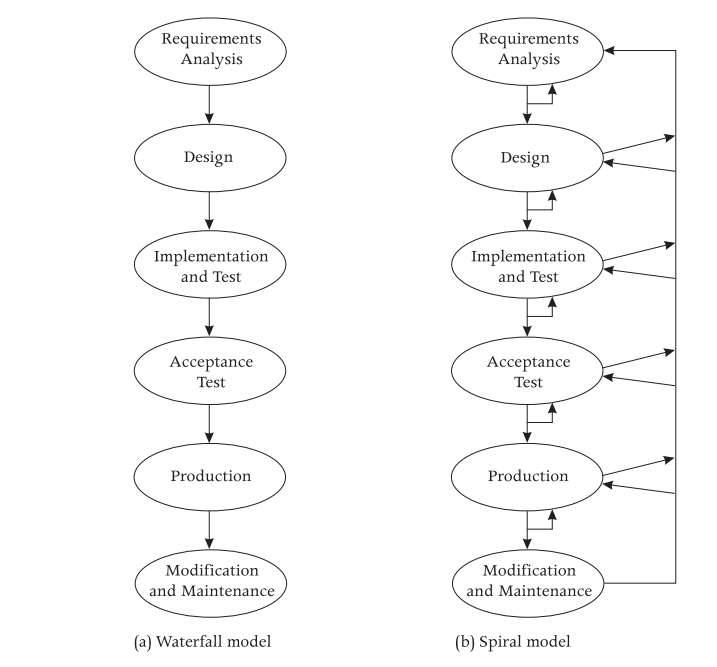
\includegraphics[width=0.8\textwidth]{media/software-life-cycle.png}
    \fonte{\citeonline{barbaraLiskov}}
    \label{fig:ciclo-vida}
\end{figure}

Para este trabalho, os requistos foram definidos no \autoref{cap:metodologia}. Da mesma forma, a fase de manutenção não será abordada, pois o foco é a construção do sistema.

\section{Design}
Esta seção utiliza como entrada os requisitos funcionais e não-funcionais definidos no \autoref{cap:metodologia} para descrever o design do sistema utilizando \acrfull{ams} e \acrfull{ddd}.

Inicialmente, é importante definir os conceitos chaves do sistema, bem como seus relacionamentos. A \autoref{fig:modelo_conceitual} ilustra as abstrações do sistema.

\begin{figure}[H]
    \centering
    \caption{Modelo conceitual do sistema}
    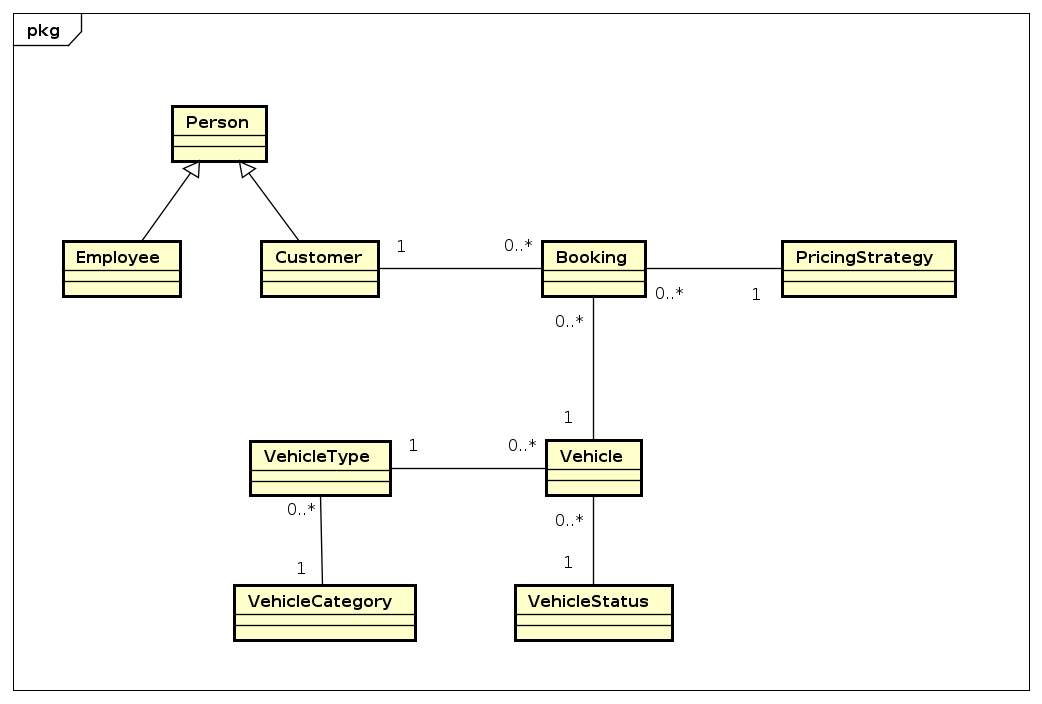
\includegraphics[width=0.8\textwidth]{media/modelo_conceitual.png}
    \fonte{o autor}
    \label{fig:modelo_conceitual}
\end{figure}

O sistema tem como componente principal a entidade \texit{Booking} que está relacionada com um \english{Vehicle} e um \english{Customer}. Cada \english{Vehicle} possui um \english{VehicleType} que tem como função agrupar veículos com características similares. Além disso, cada reserva contém uma \english{PricingStrategy} que é responsável por calcular o preço da reserva baseado em diferentes critérios. Um \english{Customer} é um subtipo de \english{Person}. Da mesma forma, o \english{Employee} é um subtipo de \english{Person}.

No contexto deste caso de uso, as abstrações \english{Booking}, \english{Vehicle}, \english{Customer}, \english{Person} e \english{Employee} possuem identidade e ciclo de vida próprios. Portanto, são entidades. Por outro lado, \english{VehicleType} e \english{PricingStrategy} são \acrfull{vo}, pois não possuem identidade própria e são imutáveis. 

\subsection{Bounded Contexts}
Após ter identificado as entidades e \acrfull{vo}, é necessário definir os \acrfull{bc} do sistema. \citeonline{evans2004ddd} define \acrshort{bc} como um limite lógico dentro do qual um modelo é consistente. Além disso, cada \acrshort{bc} possui um ou mais \english{Aggregates}. Nesse sentido, a \autoref{fig:bounded_contexts} ilustra os \acrshort{bc} do sistema.

\begin{figure}[H]
    \centering
    \caption{Bounded Contexts do sistema}
    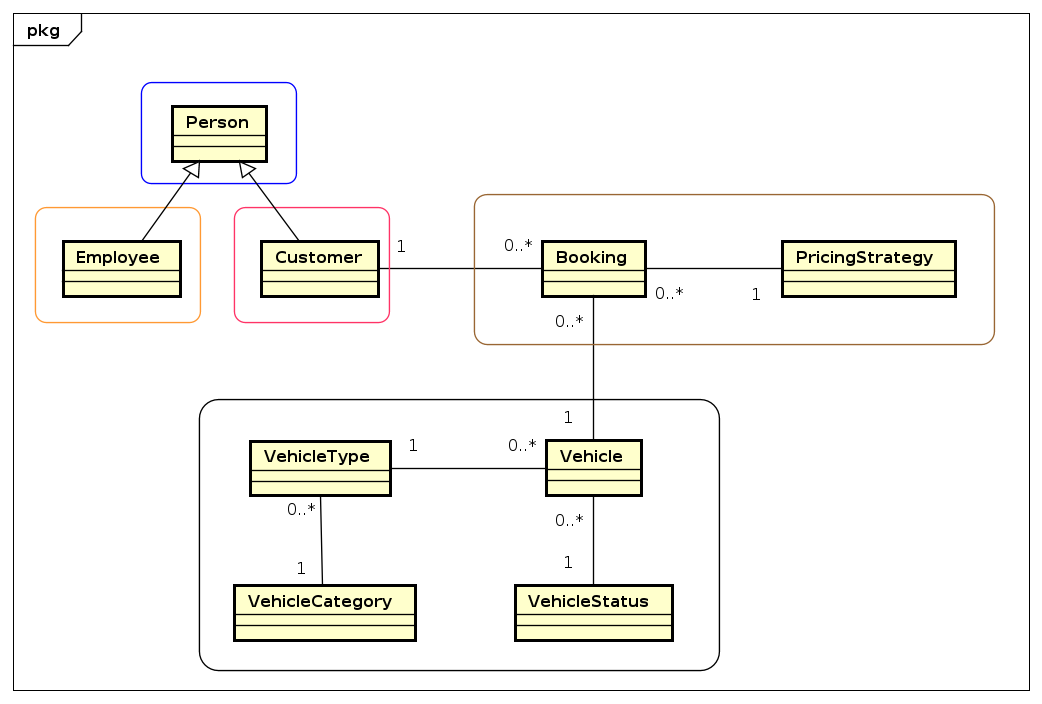
\includegraphics[width=0.8\textwidth]{media/bounded_contexts.png}
    \fonte{o autor}
    \label{fig:bounded_contexts}
\end{figure}

Ao todo, o sistema possui 5 \acrfull{bc}:
\begin{itemize}
    \item \english{Person}: Responsável por gerenciar informações de pessoas e autenticação.
    \item \english{Customer}: Realiza o gerenciamento informações de clientes.
    \item \english{Employee}: Responsável por gerenciar informações de funcionários.
    \item \english{Vehicle}: Está relacionado a estoque de veículos e tipos de veículo.
    \item \english{Booking}: Responsável por gerenciar informações de reservas e estratégias de precificação.
\end{itemize}

\subsection{Microsserviços}
Com os \acrshort{bc} definidos, é possível definir os limites de cada microsserviço. Seguindo as melhores práticas revisadas no \autoref{cap:trabalhos}, cada \acrshort{bc} é mapeado em um microsserviço. A \autoref{fig:microsservicos} ilustra a divisão dos microsserviços.

\begin{figure}[H]
    \centering
    \caption{Microsserviços do sistema}
    \fbox{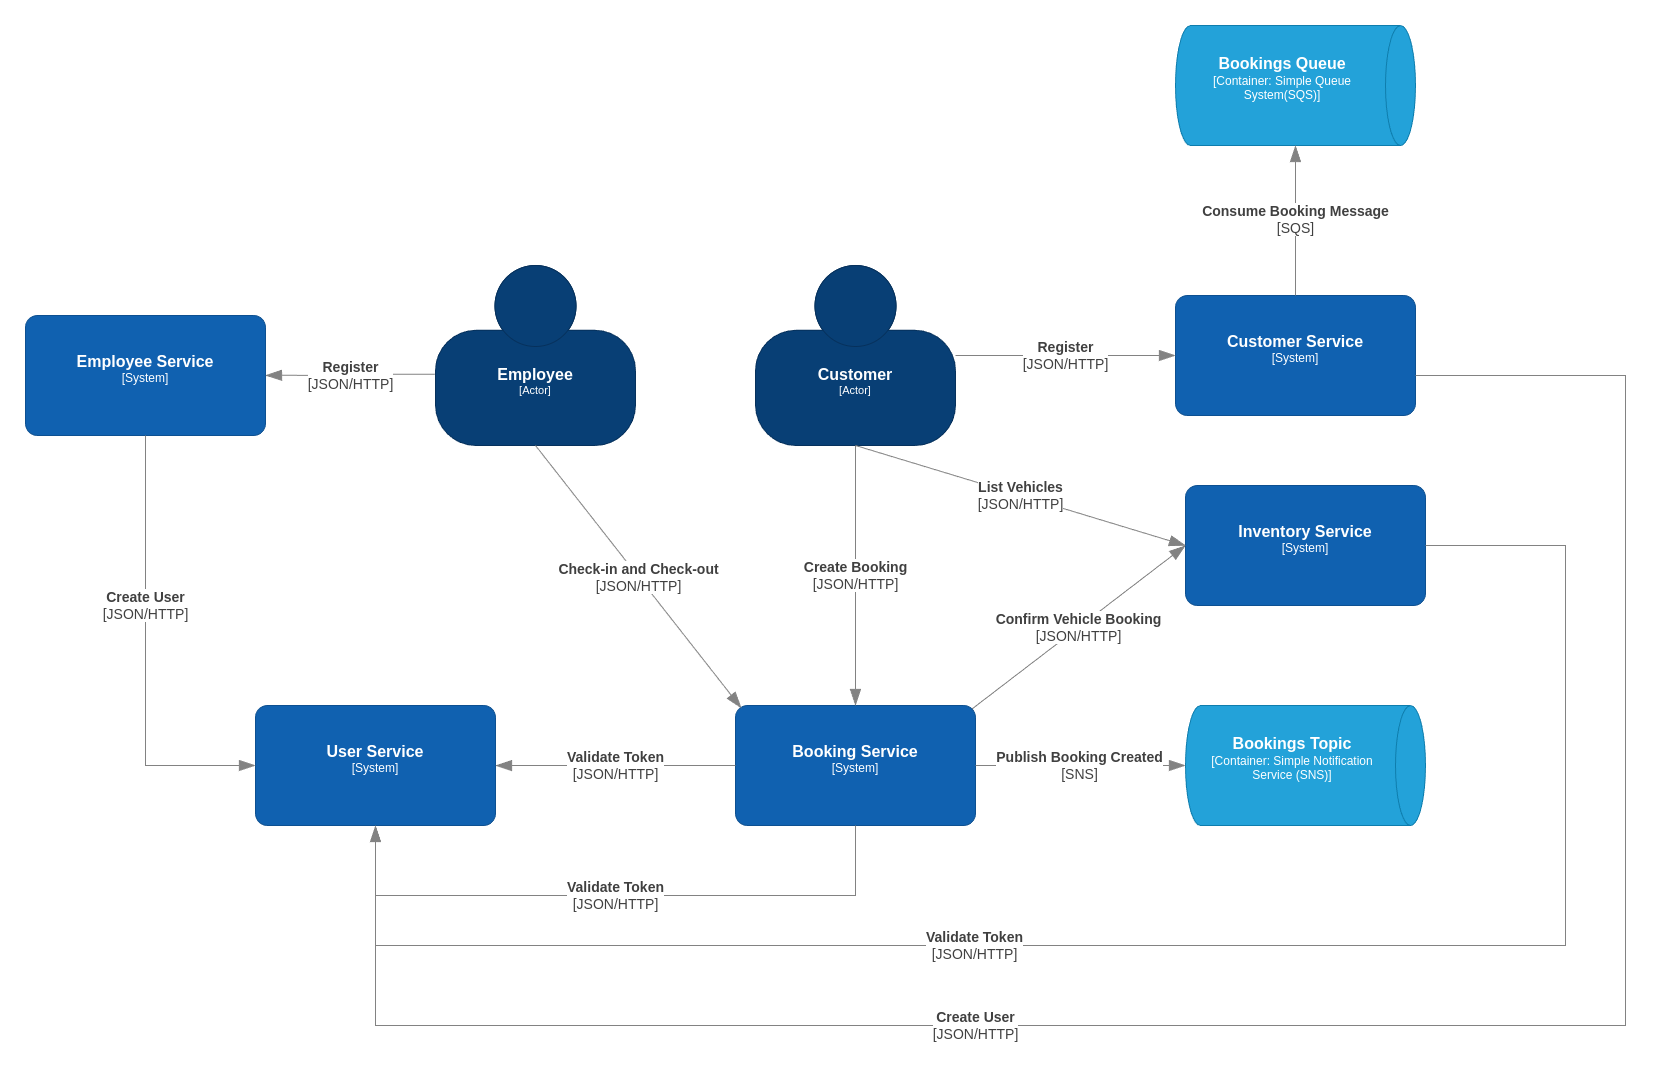
\includegraphics[width=0.8\textwidth]{media/microsservicos.png}}
    \fonte{o autor}
    \label{fig:microsservicos}
\end{figure}

Cada microsserviço é responsável por um \acrshort{bc} e possui sua própria base de dados. O \english{User Service} realiza o cadastro e login de todos usuários do sistema, além de validar \english{tokens} de autenticação. O \english{Customer Service} lida com informações de clientes. Esse serviço também consome uma fila de mensagens de reservas e atualiza um contador de reservas para cada usuário. O \english{Employee Service} gerencia informações de funcionários. O \english{Vehicle Service} trata informações de veículos como quantidade em estoque, marca, modelo, cor e tipo. Por fim, o \english{Booking Service} gerencia informações de reservas e estratégias de precificação.

\subsection{Principais casos de uso}
A seguir são detalhadas as interações entre os microsserviços para os principais casos de uso do sistema. Especificamente, são descritos os casos de uso que compõem o ciclo de vida de uma reserva ilustrado no \autoref{fig:ciclo-reserva}.

\begin{figure}[H]
    \centering
    \caption{Ciclo de vida de uma reserva}
    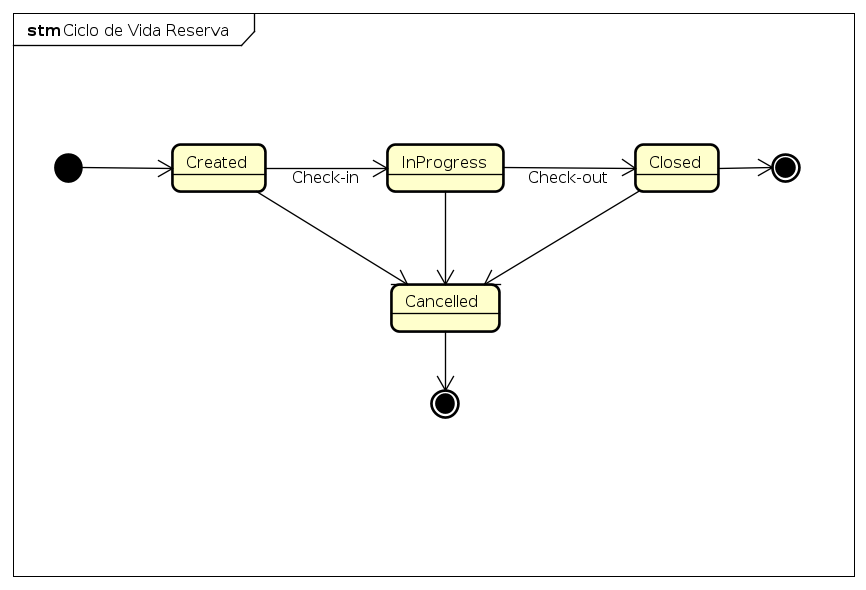
\includegraphics[width=0.8\textwidth]{media/ciclo-reserva.png}
    \fonte{o autor}
    \label{fig:ciclo-reserva}
\end{figure}

\subsubsection{Criar reserva}
A \autoref{fig:realizar-reserva} ilustra o fluxo de criação de uma reserva. Inicialmente, o cliente realiza o login no \english{User Service} e recebe um token como resposta. Em seguida, ele acessa o \english{Vehicle Service} para verificar a disponibilidade de veículos. Esse verifica se o usuário está autenticado realizando uma chamada para o \english{User Service}. Caso o usuário esteja autenticado, o \english{Vehicle Service} retorna a lista de veículos disponíveis. Posteriormente, O cliente seleciona um veículo e realiza a reserva no \english{Booking Service}. Esse serviço envia uma requisição para o \english{Inventory Service} para decrementar a quantidade de veículos disponíveis e confirmar a reserva. Por fim, o \english{Booking Service} retorna a confirmação da reserva.

\begin{figure}[H]
    \centering
    \caption{Criar reserva}
    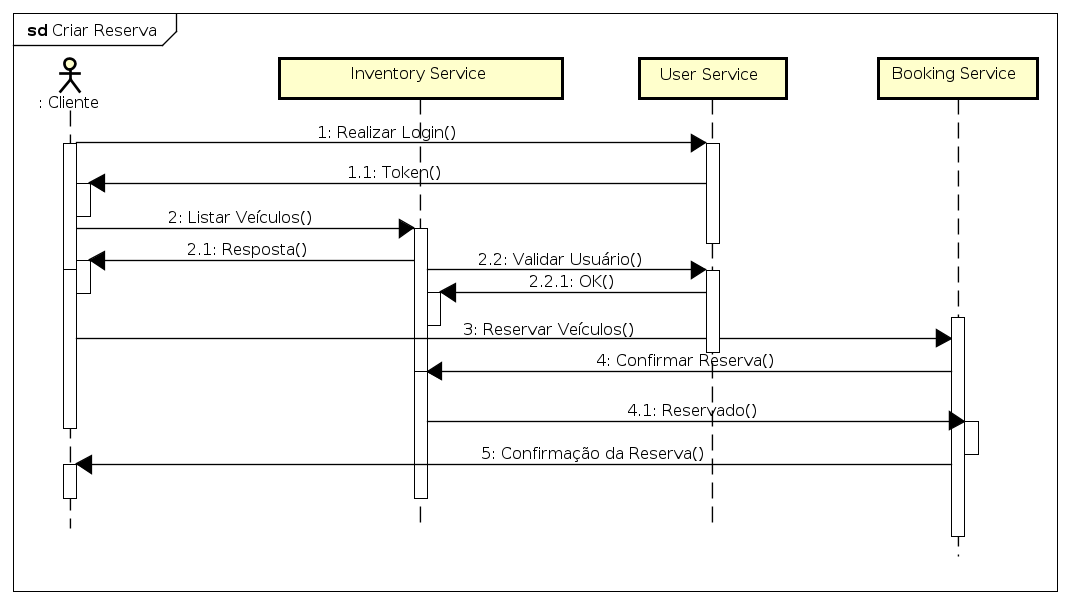
\includegraphics[width=0.8\textwidth]{media/criar-reserva.png}
    \fonte{o autor}
    \label{fig:realizar-reserva}
\end{figure}

\subsubsection{Realizar check-in}
A \autoref{fig:realizar-checkin} ilustra o fluxo de realizar um check-in. Primeiramente, o funcionário realiza o login no \english{User Service} e recebe um token como resposta. Em seguida, ele acessa o \english{Booking Service} para realizar o check-in. Esse serviço verifica se o usuário está autenticado realizando uma chamada para o \english{User Service}. Caso o usuário esteja autenticado, o \english{Booking Service} realiza o check-in e retorna a confirmação.

\begin{figure}[H]
    \centering
    \caption{Realizar check-in}
    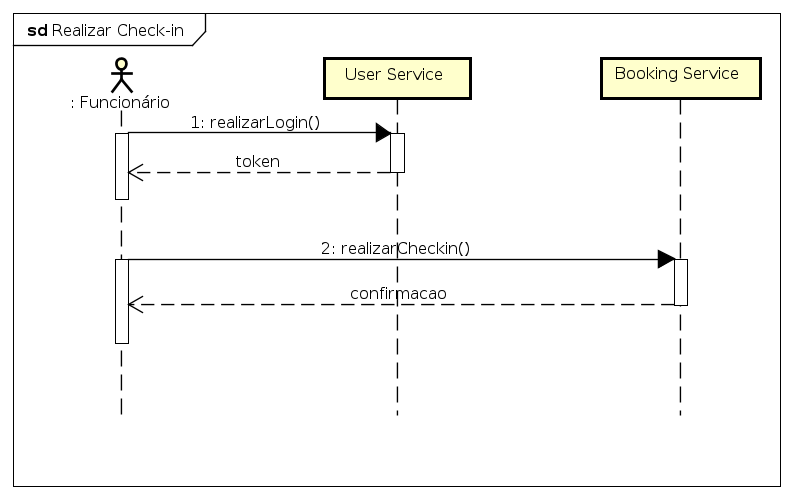
\includegraphics[width=0.8\textwidth]{media/realizar-checkin.png}
    \fonte{o autor}
    \label{fig:realizar-checkin}
\end{figure}

\subsubsection{Realizar check-out}
A \autoref{fig:realizar-checkout} ilustra o fluxo de realizar um check-out. Inicialmente, o funcionário realiza a autenticação no \english{User Service} e recebe um token como resposta. Posteriormente, ele acessa o \english{Booking Service} para realizar o check-out. Esse serviço verifica se o usuário está autenticado realizando uma chamada para o \english{User Service}. Caso o usuário esteja autenticado, o \english{Booking Service} realiza o check-out e retorna a confirmação.

\begin{figure}[H]
    \centering
    \caption{Realizar check-out}
    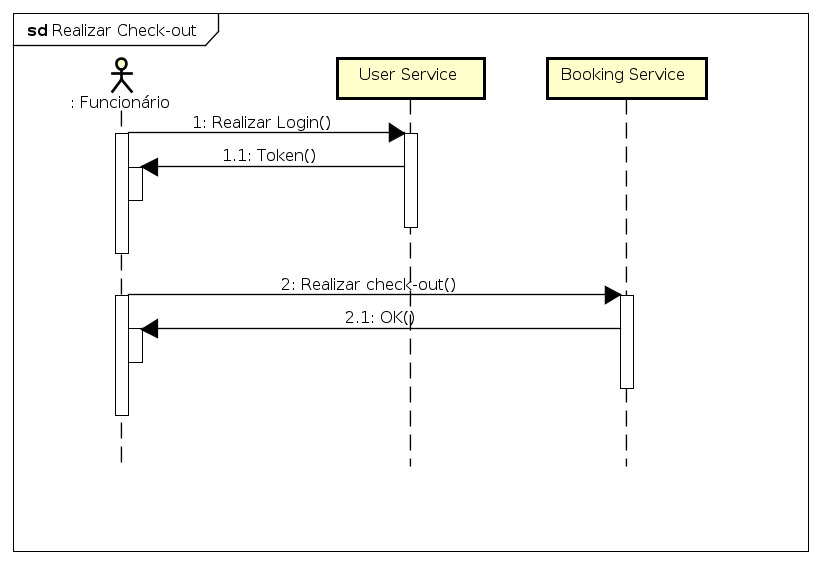
\includegraphics[width=0.8\textwidth]{media/realizar-checkout.png}
    \fonte{o autor}
    \label{fig:realizar-checkout}
\end{figure}

\subsection{User Service}
TBD

\subsection{Customer Service}
TBD

\subsection{Employee Service}
TBD

\subsection{Inventory Service}
TBD

\subsection{Booking Service}
TBD

\section{Implementação}
